\documentclass[serif]{beamer}\usepackage[]{graphicx}\usepackage[]{color}
%% maxwidth is the original width if it is less than linewidth
%% otherwise use linewidth (to make sure the graphics do not exceed the margin)
\makeatletter
\def\maxwidth{ %
  \ifdim\Gin@nat@width>\linewidth
    \linewidth
  \else
    \Gin@nat@width
  \fi
}
\makeatother

\definecolor{fgcolor}{rgb}{0.345, 0.345, 0.345}
\newcommand{\hlnum}[1]{\textcolor[rgb]{0.686,0.059,0.569}{#1}}%
\newcommand{\hlstr}[1]{\textcolor[rgb]{0.192,0.494,0.8}{#1}}%
\newcommand{\hlcom}[1]{\textcolor[rgb]{0.678,0.584,0.686}{\textit{#1}}}%
\newcommand{\hlopt}[1]{\textcolor[rgb]{0,0,0}{#1}}%
\newcommand{\hlstd}[1]{\textcolor[rgb]{0.345,0.345,0.345}{#1}}%
\newcommand{\hlkwa}[1]{\textcolor[rgb]{0.161,0.373,0.58}{\textbf{#1}}}%
\newcommand{\hlkwb}[1]{\textcolor[rgb]{0.69,0.353,0.396}{#1}}%
\newcommand{\hlkwc}[1]{\textcolor[rgb]{0.333,0.667,0.333}{#1}}%
\newcommand{\hlkwd}[1]{\textcolor[rgb]{0.737,0.353,0.396}{\textbf{#1}}}%
\let\hlipl\hlkwb

\usepackage{framed}
\makeatletter
\newenvironment{kframe}{%
 \def\at@end@of@kframe{}%
 \ifinner\ifhmode%
  \def\at@end@of@kframe{\end{minipage}}%
  \begin{minipage}{\columnwidth}%
 \fi\fi%
 \def\FrameCommand##1{\hskip\@totalleftmargin \hskip-\fboxsep
 \colorbox{shadecolor}{##1}\hskip-\fboxsep
     % There is no \\@totalrightmargin, so:
     \hskip-\linewidth \hskip-\@totalleftmargin \hskip\columnwidth}%
 \MakeFramed {\advance\hsize-\width
   \@totalleftmargin\z@ \linewidth\hsize
   \@setminipage}}%
 {\par\unskip\endMakeFramed%
 \at@end@of@kframe}
\makeatother

\definecolor{shadecolor}{rgb}{.97, .97, .97}
\definecolor{messagecolor}{rgb}{0, 0, 0}
\definecolor{warningcolor}{rgb}{1, 0, 1}
\definecolor{errorcolor}{rgb}{1, 0, 0}
\newenvironment{knitrout}{}{} % an empty environment to be redefined in TeX

\usepackage{alltt}
\usetheme{Boadilla}
\usepackage{graphicx}
\usepackage[final]{animate}
\usepackage{breqn}
\usepackage{xcolor}
\usepackage{booktabs}
\usepackage{tikz}
\usetikzlibrary{decorations.pathreplacing}
\usetikzlibrary{shapes,arrows,positioning,shadows}
\usepackage{subfig}
\usepackage{pgf}
\usepackage{caption}

% change format of enumerated lists
\setbeamertemplate{enumerate items}[default]
\setbeamertemplate{navigation symbols}{}

% macros
\newcommand{\emtxt}[1]{\textbf{\textit{{\color{mypal4} #1}}}}

% change font size for figure captions
\setbeamerfont{caption}{size=\scriptsize}

% custom colors
\definecolor{mypal1}{HTML}{F0F9E8}\definecolor{mypal2}{HTML}{BAE4BC}\definecolor{mypal3}{HTML}{7BCCC4}\definecolor{mypal4}{HTML}{43A2CA}\definecolor{mypal5}{HTML}{0868AC}

\tikzstyle{decision} = [diamond, draw, text width=6em, text badly centered, inner sep = 2pt, top color=white, bottom color=mypal3, drop shadow]
\tikzstyle{block} = [rectangle, draw, text width=10em, text centered, rounded corners, minimum height=3em, minimum width=8em, top color = white, bottom color=mypal4,  drop shadow]
\tikzstyle{declare} = [rectangle, draw, text width=10em, text centered, minimum height=3em, minimum width=8em, top color = white, bottom color=mypal5,  drop shadow]

% knitr setup


% dependent data


% get online bib file


\setbeamercolor{title}{fg=mypal5} % main title
\setbeamercolor{frametitle}{fg=mypal4, bg=mypal2} % frame titles
\setbeamercolor{structure}{fg=mypal4} % bottom banner
\setbeamercolor{normal text}{fg=mypal5}
\usebackgroundtemplate{\includegraphics[height=\paperheight,width=\paperwidth]{fig/back_tmp.pdf}}
\IfFileExists{upquote.sty}{\usepackage{upquote}}{}
\begin{document}

\title[Open science for restoration]{\textbf{Use of open science to inform restoration projects in estuaries: A Tampa Bay example}}
\author[Beck et al.]{Marcus W. Beck$^1$, Ed Sherwood, Kirsten Dorans, Jessica Renee Henkel, Kathryn Ireland, Patricia Varela}

\institute[SCCWRP]{$^1$Southern California Coastal Water Research Project, Costa Mesa, CA \href{mailto:marcusb@sccwrp.org}{marcusb@sccwrp.org}, Phone: 714-755-3217}

\date{April 23, 2018}

% \titlegraphic{
% }

%%%%%%
\begin{frame}[shrink]
\vspace{0.2in}
\titlepage
\end{frame}

\section{Background}

%%%%%%
\begin{frame}{{$\vcenter{\hbox{\includegraphics[width=0.07\paperwidth]{fig/sccwrp_logo.png}}}$\hspace{0.07in}\textbf{Open science workflow}}}
\centerline{\includegraphics[width=0.85\textwidth]{fig/scienceflow.png}}
\vfill
\tiny
Modified from \href{https://esajournals.onlinelibrary.wiley.com/doi/full/10.1890/ES14-00402.1}{Hampton et al. 2015. The Tao of open science for ecology. Ecosphere 6(7):1-13.}
\end{frame}

%%%%%%
\begin{frame}[t]{Final thoughts}{}
{\large \emtxt{Open Science for Synthesis: Gulf Research Program}}
\begin{columns}
\begin{column}{0.5\textwidth}
July 10 - July 28, 2017\\
NCEAS, Santa Barbara, CA 
\end{column}
\begin{column}{0.5\textwidth}
\hfill \includegraphics[width = \textwidth]{fig/nceas_full.png}
\end{column}
\end{columns}
\vspace{0.1in}
\begin{columns}
\begin{column}{0.5\textwidth}
\centerline{\fbox{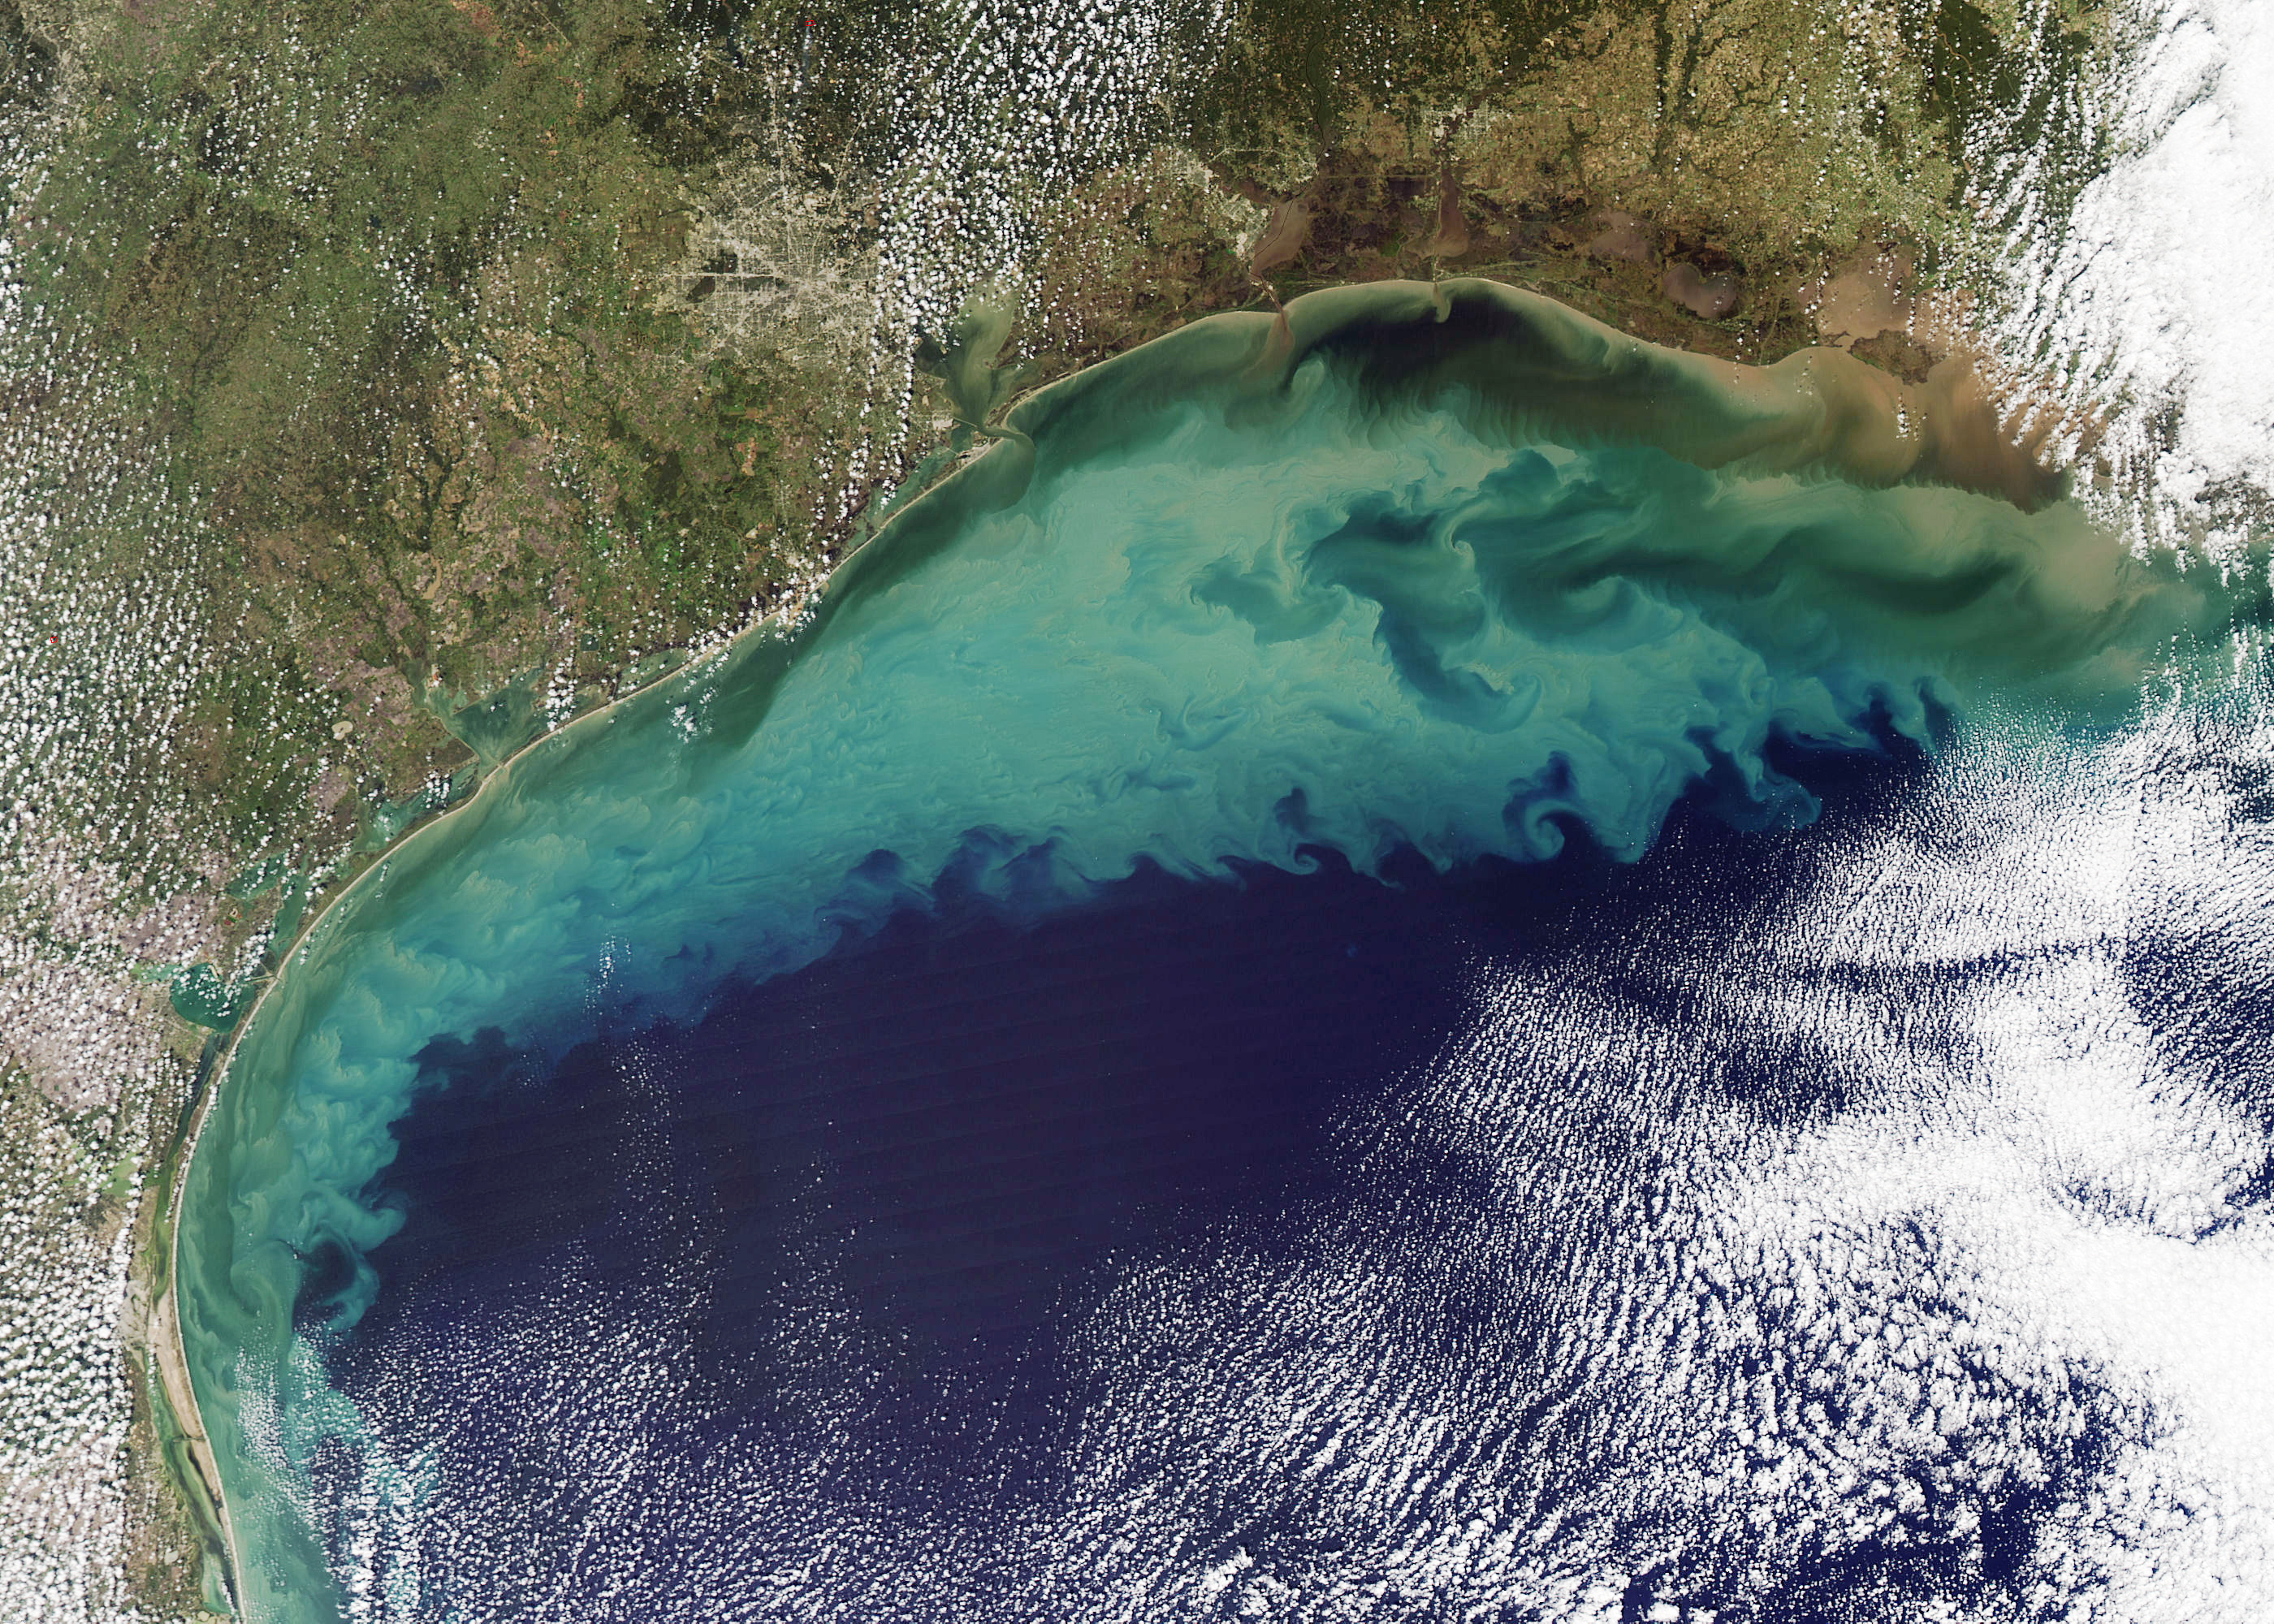
\includegraphics[width = 0.85\textwidth]{fig/gom.jpg}}}
\end{column}
\begin{column}{0.5\textwidth}
\centerline{\fbox{\includegraphics[width = 0.65\textwidth]{fig/ossgrp.jpg}}}
\end{column}
\end{columns}
\end{frame}

%%%%%%
\begin{frame}{{$\vcenter{\hbox{\includegraphics[width=0.07\paperwidth]{fig/sccwrp_logo.png}}}$\hspace{0.07in}\textbf{Open science workflow}}}
{\large \emtxt{Open Science for Synthesis: Gulf Research Program}}
\begin{columns}
\begin{column}{0.5\textwidth}
July 10 - July 28, 2017\\
NCEAS, Santa Barbara, CA 
\end{column}
\begin{column}{0.5\textwidth}
\hfill \includegraphics[width = \textwidth]{fig/nceas_full.png}
\end{column}
\end{columns}
\vspace{0.1in}
\vfill
\centerline{\url{https://nceas.github.io/oss-2017/lessons.html}}
\begin{itemize}
\item Collaboration modes and technologies, virtual collaboration
\item Data management, preservation, and sharing
\item Data manipulation, integration, and exploration
\item Scientific workflows and reproducible research
\item Programming using agile and sustainable software practices
\item Data analysis and modeling
\item Communicating results to broad communities
\end{itemize}
\vfill
\end{frame}

%%%%%%
\begin{frame}{{$\vcenter{\hbox{\includegraphics[width=0.07\paperwidth]{fig/sccwrp_logo.png}}}$\hspace{0.07in}\textbf{Today's talk}}}
\onslide<+->
Our experience using the open science workflow to inform restoration projects in estuaries \\~\\
\onslide<+->
Can we use disparate data to prioritize future restoration projects aimed at improving water quality? \\~\\
\begin{itemize}
\item<+-> \emtxt{Synthesize} data in space and time to evaluate cumulative effects of restoration projects\\~\\
\item<+-> \emtxt{Develop} a Bayesian Decision Network with empirical observations to evaluate likelihood of potential outcomes \\~\\
\item<+-> \emtxt{Apply} the Decision Network to guide expectations for future restoration projects
\end{itemize}
\end{frame}

%%%%%%
\begin{frame}{{$\vcenter{\hbox{\includegraphics[width=0.07\paperwidth]{fig/sccwrp_logo.png}}}$\hspace{0.07in}\textbf{Tampa Bay - from gross to less gross}}}
\begin{columns}
\begin{column}{0.5\textwidth}
\onslide<+->
\begin{center}
\includegraphics[width=0.7\textwidth]{fig/TB_Algae.png}\\~\\
\includegraphics[width=0.7\textwidth]{fig/post_rest_sh.jpg}\\~\\
\end{center}
\end{column}
\begin{column}{0.5\textwidth}
\emtxt{Past:}
\begin{itemize}
\item Mid-1970s N load 8.2$\times$10$^6$ yr$^{-1}$ {\footnotesize \cite{Greening06}}
\item Elevated chl-a concentrations
\item Increased occurrence of HABs
\end{itemize}
\onslide<+->
\emtxt{Present:}
\begin{itemize}
\item 2016 seagrass at ~17k ha {\footnotesize \cite{Sherwood17}}
\item Reductions in nutrient load, chlorophyll
\item Increase in water clarity {\footnotesize \cite{Morrison06,Beck17c}}
\end{itemize}
\end{column}
\end{columns}
\end{frame}

%%%%%%
\begin{frame}{{$\vcenter{\hbox{\includegraphics[width=0.07\paperwidth]{fig/sccwrp_logo.png}}}$\hspace{0.07in}\textbf{Tampa Bay - open data sources}}}
\begin{columns}
\begin{column}{0.5\textwidth}
\onslide<+->
\begin{center}
\includegraphics[width=0.95\textwidth]{fig/tbrest_map.pdf}
\end{center}
\end{column}
\begin{column}{0.5\textwidth}
\begin{itemize}
\item \emtxt{Water quality} monitoring dataset - 1974 to present, ~ 500 obs. per site \\~\\
\item<+-> \emtxt{Restoration projects} dataset - 500 projects since 1971, habitat and water infrastructure projects
\end{itemize}
\end{column}
\end{columns}
\onslide<+->
\begin{center}
Despite considerable \emtxt{investments} in restoration, \emtxt{effectiveness evaluation} continues to elude practitioners at geographic scales {\footnotesize \cite{Diefenderfer16}}
\end{center}
\end{frame}

%%%%%%
\begin{frame}{{$\vcenter{\hbox{\includegraphics[width=0.07\paperwidth]{fig/sccwrp_logo.png}}}$\hspace{0.07in}\textbf{Data munging with open source tools}}}
Empirical relationship fed into decision support tool
\end{frame}

%%%%%%
\begin{frame}{{$\vcenter{\hbox{\includegraphics[width=0.07\paperwidth]{fig/sccwrp_logo.png}}}$\hspace{0.07in}\textbf{Open science workflow}}}
\centerline{\includegraphics[width=0.85\textwidth]{fig/scienceflow.png}}
\vfill
\tiny
Modified from \cite{Hampton15}
\end{frame}

%%%%%%
\begin{frame}{{$\vcenter{\hbox{\includegraphics[width=0.07\paperwidth]{fig/sccwrp_logo.png}}}$\hspace{0.07in}\textbf{Open science workflow}}}
What aspects of our project used and benefitted from open science?
\begin{itemize}
\item Early idea conception
\item Long distance collaboration
\item Transparent and reproducible analysis
\end{itemize}
\centerline{Teach a scientist to fish...}
\end{frame}

%%%%%%
\section{References}
\begin{frame}[t,shrink]{\textbf{References}}
\tiny
\setbeamertemplate{bibliography item}{}
\bibliographystyle{apalike_mine}
\bibliography{refs}
\end{frame}

\end{document}
